\begin{figure}[h] 
\centering 
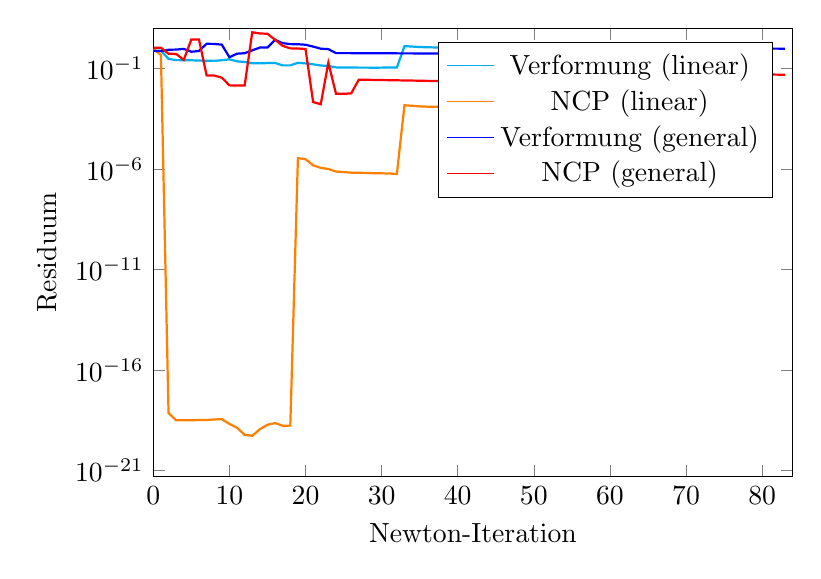
\begin{tikzpicture}[every plot/.append style={thick}] 
\begin{axis}[ 
label style={font=\normalsize}, 
xlabel={Newton-Iteration}, 
ylabel={Residuum}, 
xmin=0, xmax=84, 
ymode=log, 
ymin=0, ymax=10, 
width=0.8\textwidth, 
height=0.6\textwidth, 
legend pos=north east, 
legend style={cells={align=left}}, 
grid style=dashed, 
] 
\addplot[ 
color=cyan, 
] 
coordinates { 
(0, 7.70e-01)(1, 7.62e-01)(2, 3.00e-01)(3, 2.60e-01)(4, 2.57e-01)(5, 2.54e-01)(6, 2.47e-01)(7, 2.41e-01)(8, 2.38e-01)(9, 2.56e-01)(10, 2.84e-01)(11, 2.26e-01)(12, 2.11e-01)(13, 1.81e-01)(14, 1.79e-01)(15, 1.85e-01)(16, 1.88e-01)(17, 1.42e-01)(18, 1.42e-01)(19, 1.91e-01)(20, 1.78e-01)(21, 1.60e-01)(22, 1.40e-01)(23, 1.33e-01)(24, 1.13e-01)(25, 1.11e-01)(26, 1.11e-01)(27, 1.10e-01)(28, 1.10e-01)(29, 1.09e-01)(30, 1.10e-01)(31, 1.11e-01)(32, 1.10e-01)(33, 1.28e+00)(34, 1.23e+00)(35, 1.16e+00)(36, 1.13e+00)(37, 1.11e+00)(38, 1.08e+00)(39, 4.75e-01)(40, 4.69e-01)(41, 4.85e-01)(42, 4.42e-01)(43, 3.65e-01)}; 
\addlegendentry{Verformung (linear)} 
\addplot[ 
color=orange, 
] 
coordinates { 
(0, 9.36e-01)(1, 4.68e-01)(2, 7.32e-19)(3, 3.18e-19)(4, 3.25e-19)(5, 3.22e-19)(6, 3.30e-19)(7, 3.30e-19)(8, 3.52e-19)(9, 3.62e-19)(10, 2.12e-19)(11, 1.36e-19)(12, 6.06e-20)(13, 5.42e-20)(14, 1.15e-19)(15, 1.92e-19)(16, 2.32e-19)(17, 1.71e-19)(18, 1.74e-19)(19, 3.48e-06)(20, 3.05e-06)(21, 1.52e-06)(22, 1.14e-06)(23, 9.99e-07)(24, 7.49e-07)(25, 7.03e-07)(26, 6.59e-07)(27, 6.48e-07)(28, 6.38e-07)(29, 6.18e-07)(30, 6.09e-07)(31, 5.99e-07)(32, 5.62e-07)(33, 1.48e-03)(34, 1.39e-03)(35, 1.30e-03)(36, 1.26e-03)(37, 1.24e-03)(38, 1.23e-03)(39, 9.90e-04)(40, 9.74e-04)(41, 9.73e-04)(42, 9.57e-04)(43, 9.51e-04)}; 
\addlegendentry{NCP (linear)} 
\addplot[ 
color=blue, 
] 
coordinates { 
(0, 7.36e-01)(1, 7.27e-01)(2, 8.54e-01)(3, 8.67e-01)(4, 9.40e-01)(5, 6.78e-01)(6, 7.39e-01)(7, 1.68e+00)(8, 1.66e+00)(9, 1.53e+00)(10, 3.61e-01)(11, 5.42e-01)(12, 5.72e-01)(13, 7.97e-01)(14, 1.09e+00)(15, 1.09e+00)(16, 2.66e+00)(17, 1.81e+00)(18, 1.62e+00)(19, 1.60e+00)(20, 1.51e+00)(21, 1.22e+00)(22, 9.61e-01)(23, 9.14e-01)(24, 5.79e-01)(25, 5.79e-01)(26, 5.77e-01)(27, 5.74e-01)(28, 5.71e-01)(29, 5.69e-01)(30, 5.67e-01)(31, 5.65e-01)(32, 5.63e-01)(33, 5.62e-01)(34, 5.61e-01)(35, 5.58e-01)(36, 5.56e-01)(37, 5.54e-01)(38, 5.52e-01)(39, 5.50e-01)(40, 5.49e-01)(41, 5.47e-01)(42, 5.53e-01)(43, 1.14e+00)(44, 1.13e+00)(45, 1.12e+00)(46, 1.10e+00)(47, 1.09e+00)(48, 1.09e+00)(49, 1.08e+00)(50, 1.07e+00)(51, 1.07e+00)(52, 1.06e+00)(53, 1.06e+00)(54, 1.06e+00)(55, 1.06e+00)(56, 1.06e+00)(57, 1.06e+00)(58, 1.06e+00)(59, 1.06e+00)(60, 1.06e+00)(61, 1.06e+00)(62, 1.06e+00)(63, 1.06e+00)(64, 1.06e+00)(65, 1.07e+00)(66, 1.06e+00)(67, 1.05e+00)(68, 1.05e+00)(69, 1.04e+00)(70, 1.03e+00)(71, 1.03e+00)(72, 1.02e+00)(73, 1.02e+00)(74, 1.01e+00)(75, 1.00e+00)(76, 9.98e-01)(77, 9.93e-01)(78, 9.87e-01)(79, 9.83e-01)(80, 9.76e-01)(81, 9.72e-01)(82, 9.67e-01)(83, 9.60e-01)}; 
\addlegendentry{Verformung (general)} 
\addplot[ 
color=red, 
] 
coordinates { 
(0, 1.08e+00)(1, 1.07e+00)(2, 5.42e-01)(3, 5.25e-01)(4, 2.67e-01)(5, 2.79e+00)(6, 2.74e+00)(7, 4.52e-02)(8, 4.45e-02)(9, 3.48e-02)(10, 1.44e-02)(11, 1.42e-02)(12, 1.40e-02)(13, 6.27e+00)(14, 5.49e+00)(15, 5.31e+00)(16, 2.66e+00)(17, 1.33e+00)(18, 9.97e-01)(19, 9.81e-01)(20, 9.24e-01)(21, 2.13e-03)(22, 1.66e-03)(23, 1.95e-01)(24, 5.56e-03)(25, 5.47e-03)(26, 5.76e-03)(27, 2.77e-02)(28, 2.73e-02)(29, 2.69e-02)(30, 2.65e-02)(31, 2.61e-02)(32, 2.57e-02)(33, 2.53e-02)(34, 2.49e-02)(35, 2.46e-02)(36, 2.41e-02)(37, 2.39e-02)(38, 2.34e-02)(39, 2.31e-02)(40, 2.27e-02)(41, 2.25e-02)(42, 2.18e-02)(43, 2.12e-02)(44, 2.05e-02)(45, 1.21e-01)(46, 1.17e-01)(47, 1.14e-01)(48, 1.10e-01)(49, 1.07e-01)(50, 1.03e-01)(51, 1.00e-01)(52, 9.70e-02)(53, 9.39e-02)(54, 9.10e-02)(55, 8.82e-02)(56, 8.54e-02)(57, 8.28e-02)(58, 8.02e-02)(59, 7.77e-02)(60, 7.53e-02)(61, 7.29e-02)(62, 7.07e-02)(63, 6.85e-02)(64, 6.63e-02)(65, 6.43e-02)(66, 6.33e-02)(67, 6.23e-02)(68, 6.13e-02)(69, 6.04e-02)(70, 5.94e-02)(71, 5.85e-02)(72, 5.76e-02)(73, 5.67e-02)(74, 5.58e-02)(75, 5.49e-02)(76, 5.41e-02)(77, 5.33e-02)(78, 5.24e-02)(79, 5.16e-02)(80, 5.08e-02)(81, 5.00e-02)(82, 4.92e-02)(83, 4.85e-02)}; 
\addlegendentry{NCP (general)} 
\end{axis} 
\end{tikzpicture} 
\caption{Residuen des Stoffgesetzes 'St.Venant' mit Hinderniss 'Hut' und 2178 Freiheitsgraden für die Verschiebung.} 
\label{fiq:St.Venant_Hut_level4} 
\end{figure} 
